\subsection{Overview}
When we first started designing our data collection interface, we wanted to collect sketches for prompts similar to the ones used in DALL-E \citep{dallePaper}: creative composition of attributes and objects that are not commonly associated. 
For example, \textit{an evil cup of bubble tea} and \textit{happy moon}. 
In addition to sketches, we also require annotators to decompose their drawings into steps and provide descriptions for each step. We hope to discover combination of simple shapes like examples in Figure \ref{introduction.composition}, and because the imaginative prompts would result in creative sketches, the part descriptions would also be interesting\pdfmarkupcomment[color=yellow]{, like}{want to talk about the YouTube example}.     

We deploy the data collection interface on Amazon Mechanical Turk (AMT), which is a crowdsourcing website that hosts different machine learning annotation tasks. In the remaining text, we use the word \textit{turker} to refer to annotators we recruit on AMT; we will also use the word \textit{HIT}, Human Intelligence Task, to refer to a task hosted on AMT. Please refer to \href{https://www.mturk.com/worker/help#:~:text=A%20Human%20Intelligence%20Task%2C%20or,be%20completed%20by%20Worker%20customers.}{AMT FAQs} for official definition and answers to questions related to AMT. 
 
For each HIT, we need to design: (1) instruction and requirements explaining the dos and don'ts; (2) qualification task to train turkers to provide high-quality annotations; (3) the main interface for data collection. 
% Compared to Version 0, which we only dabbled with \ref{v1_sec_1} in the above list, we went through all three stages for Version 1 and eventually deployed a pilot.
After deploying the pilot, we realized a few major problems with this design. Firstly, due to the subjective nature of sketching, although the sketches are very creative, it was hard to understand how some annotators are illustrating the given prompts. Moreover, turkers are taking more than 30 minutes for each task, and, most importantly, many descriptions do not align with the drawn objects, making the data difficult to use for model learning. For example, in one step, an annotator drew the entire cat face, but they only annotated \textit{big eyes}.      

\subsection{Interface Design}

\subsubsection{Main Task Interface}
% Compare to version 0, we make the following changes to the task interface: 
% \begin{enumerate}
%     \item Since turkers are paid based on time spent on the task, we decided to forsake the functionality related to the recording and replaying the drawing board.
%     \item Since we decide to not limit the drawings to be compositions of basic geometric objects, we removed the step to select primitive shape preceding drawing each component.
% \end{enumerate}

\begin{figure*}[!htb]
\begin{subfigure}{\textwidth}
    \centering
    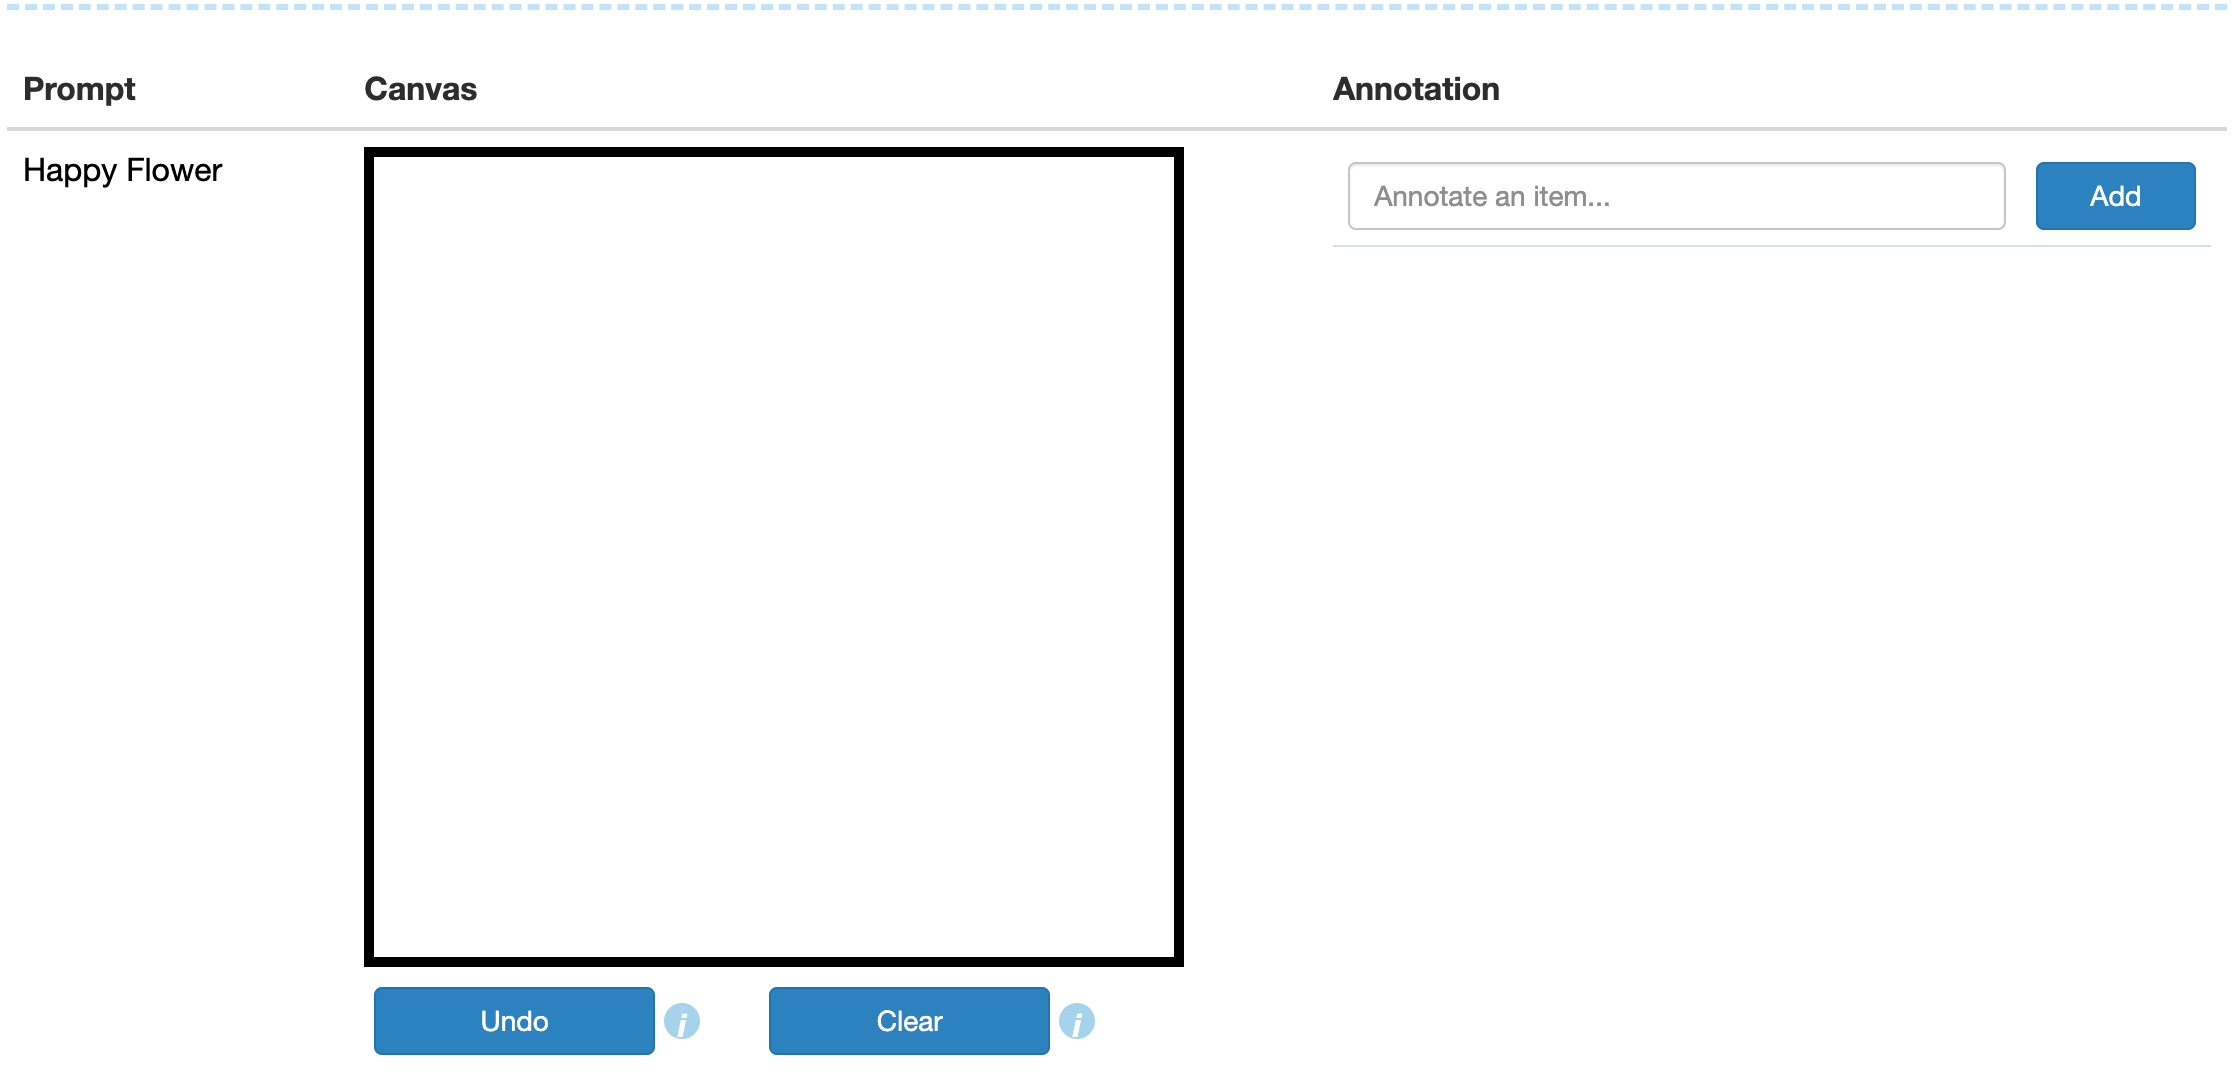
\includegraphics[width=.75\linewidth]{data_collection/v1_empty_table.png}  
\end{subfigure}
\newline
\begin{subfigure}{\textwidth}
    \centering
    % include third image
    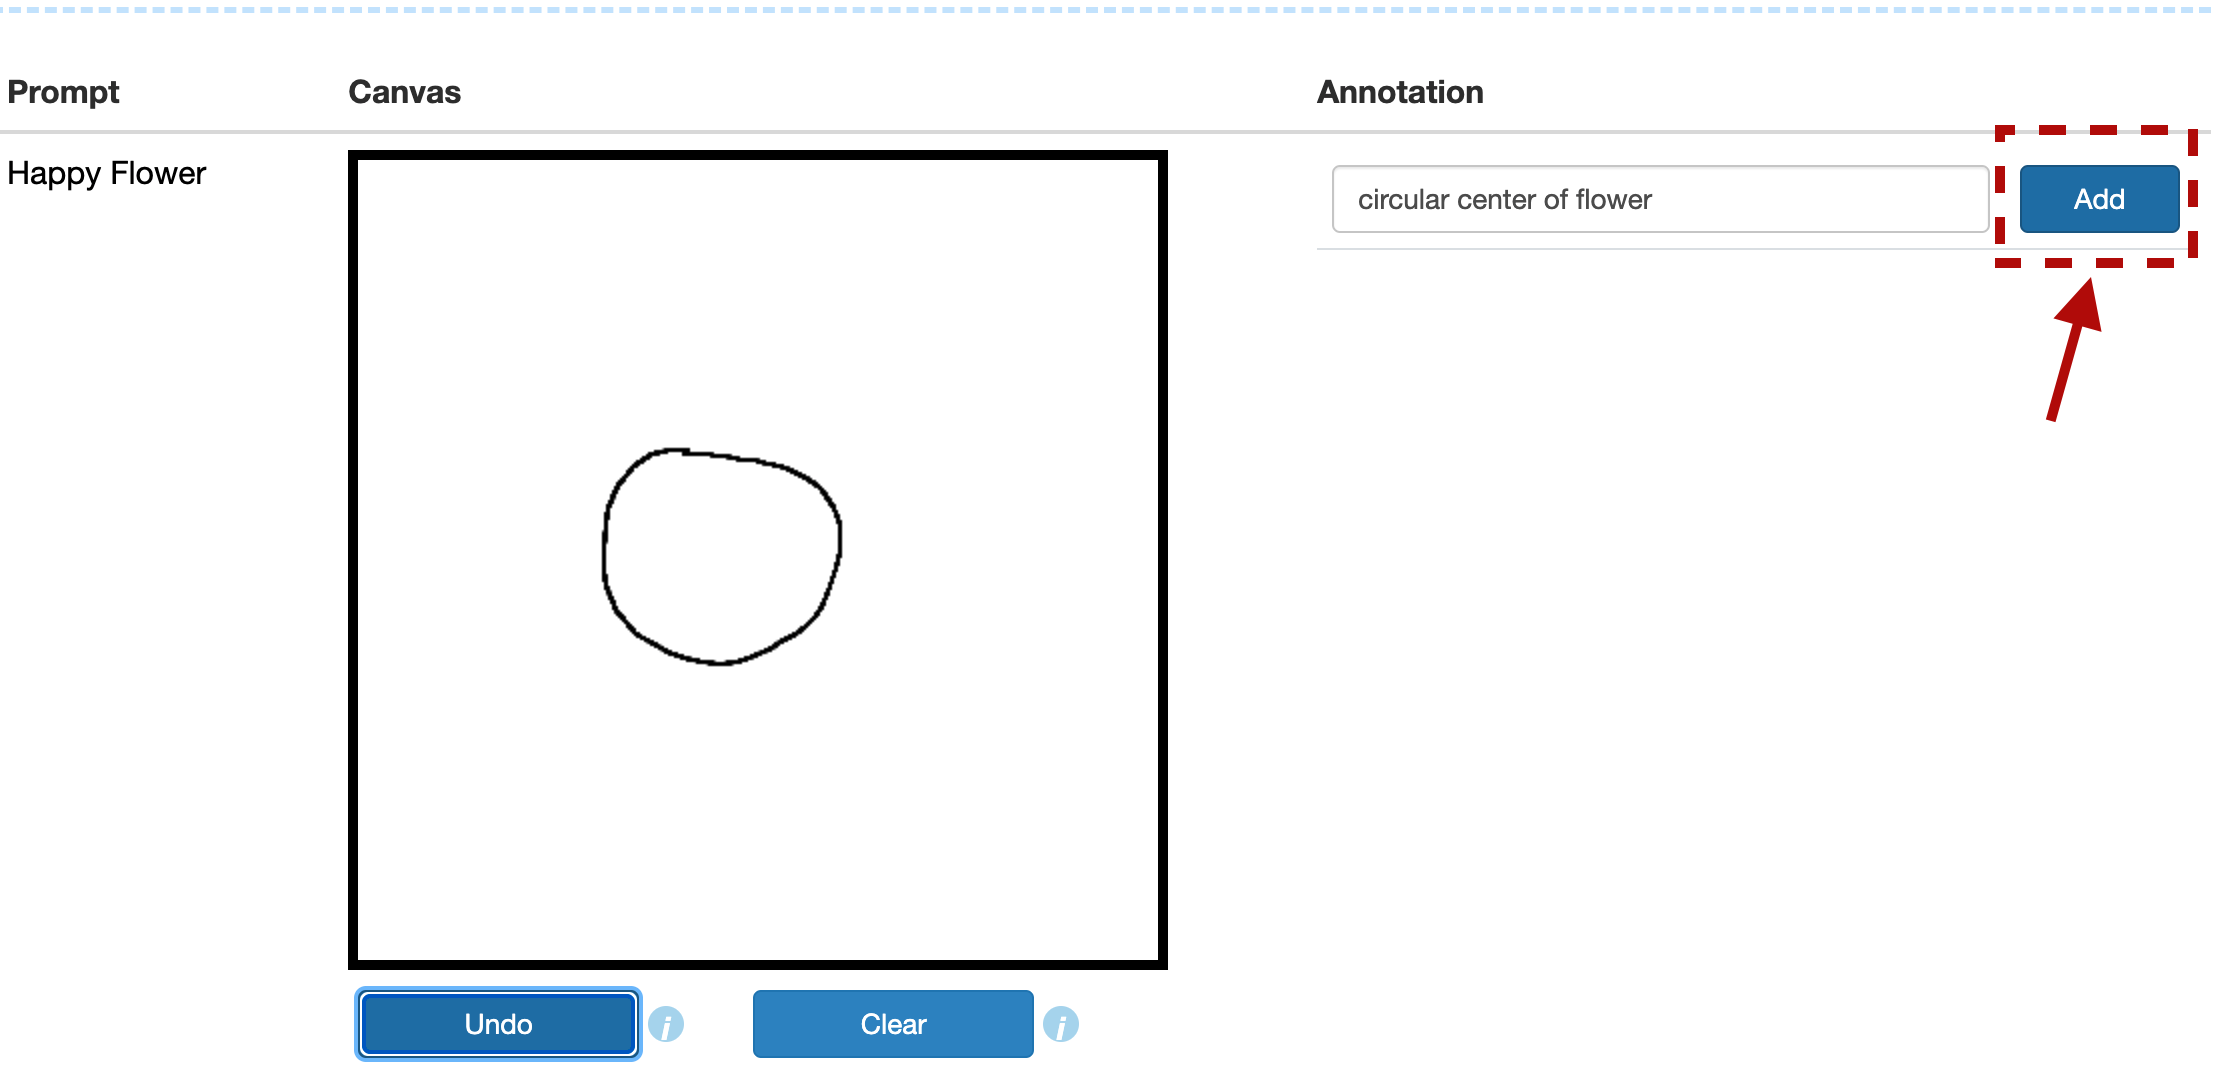
\includegraphics[width=.75\linewidth]{data_collection/v1_before_enter_text.png}  
\end{subfigure}
\newline
\begin{subfigure}{\textwidth}
    \centering
    % include third image
    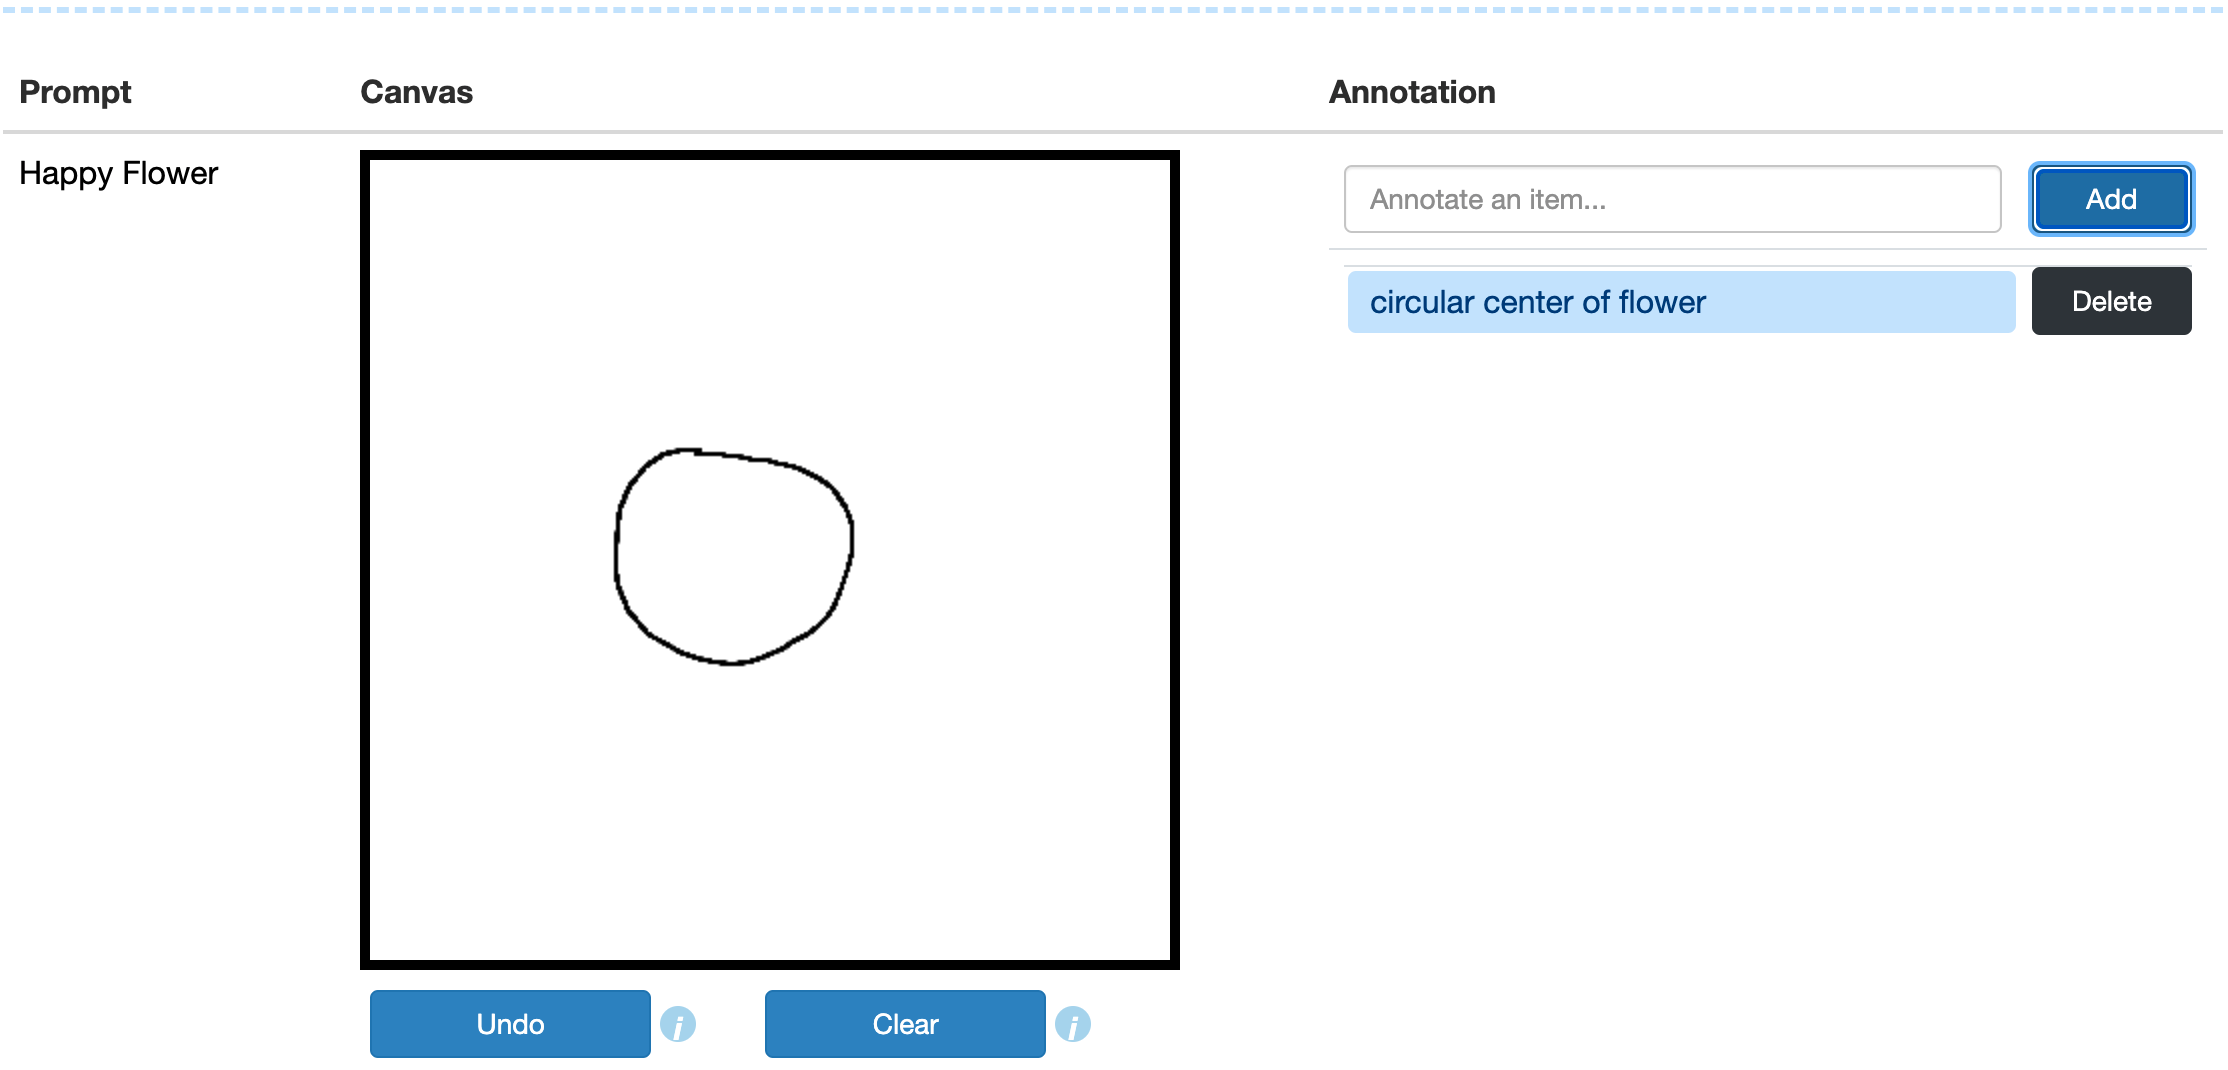
\includegraphics[width=.75\linewidth]{data_collection/v1_after_enter_text.png}  
\end{subfigure}
\caption{A typical annotation process. Top: interface at the start of annotation. Middle: before adding text descriptions for the drawing; red arrow and box show where to click to add text. Bottom: after adding text descriptions for the flower sketch.}
\label{v1.main_task.1}
\end{figure*}

\begin{figure*}[!htb]
\begin{subfigure}{\textwidth}
\centering
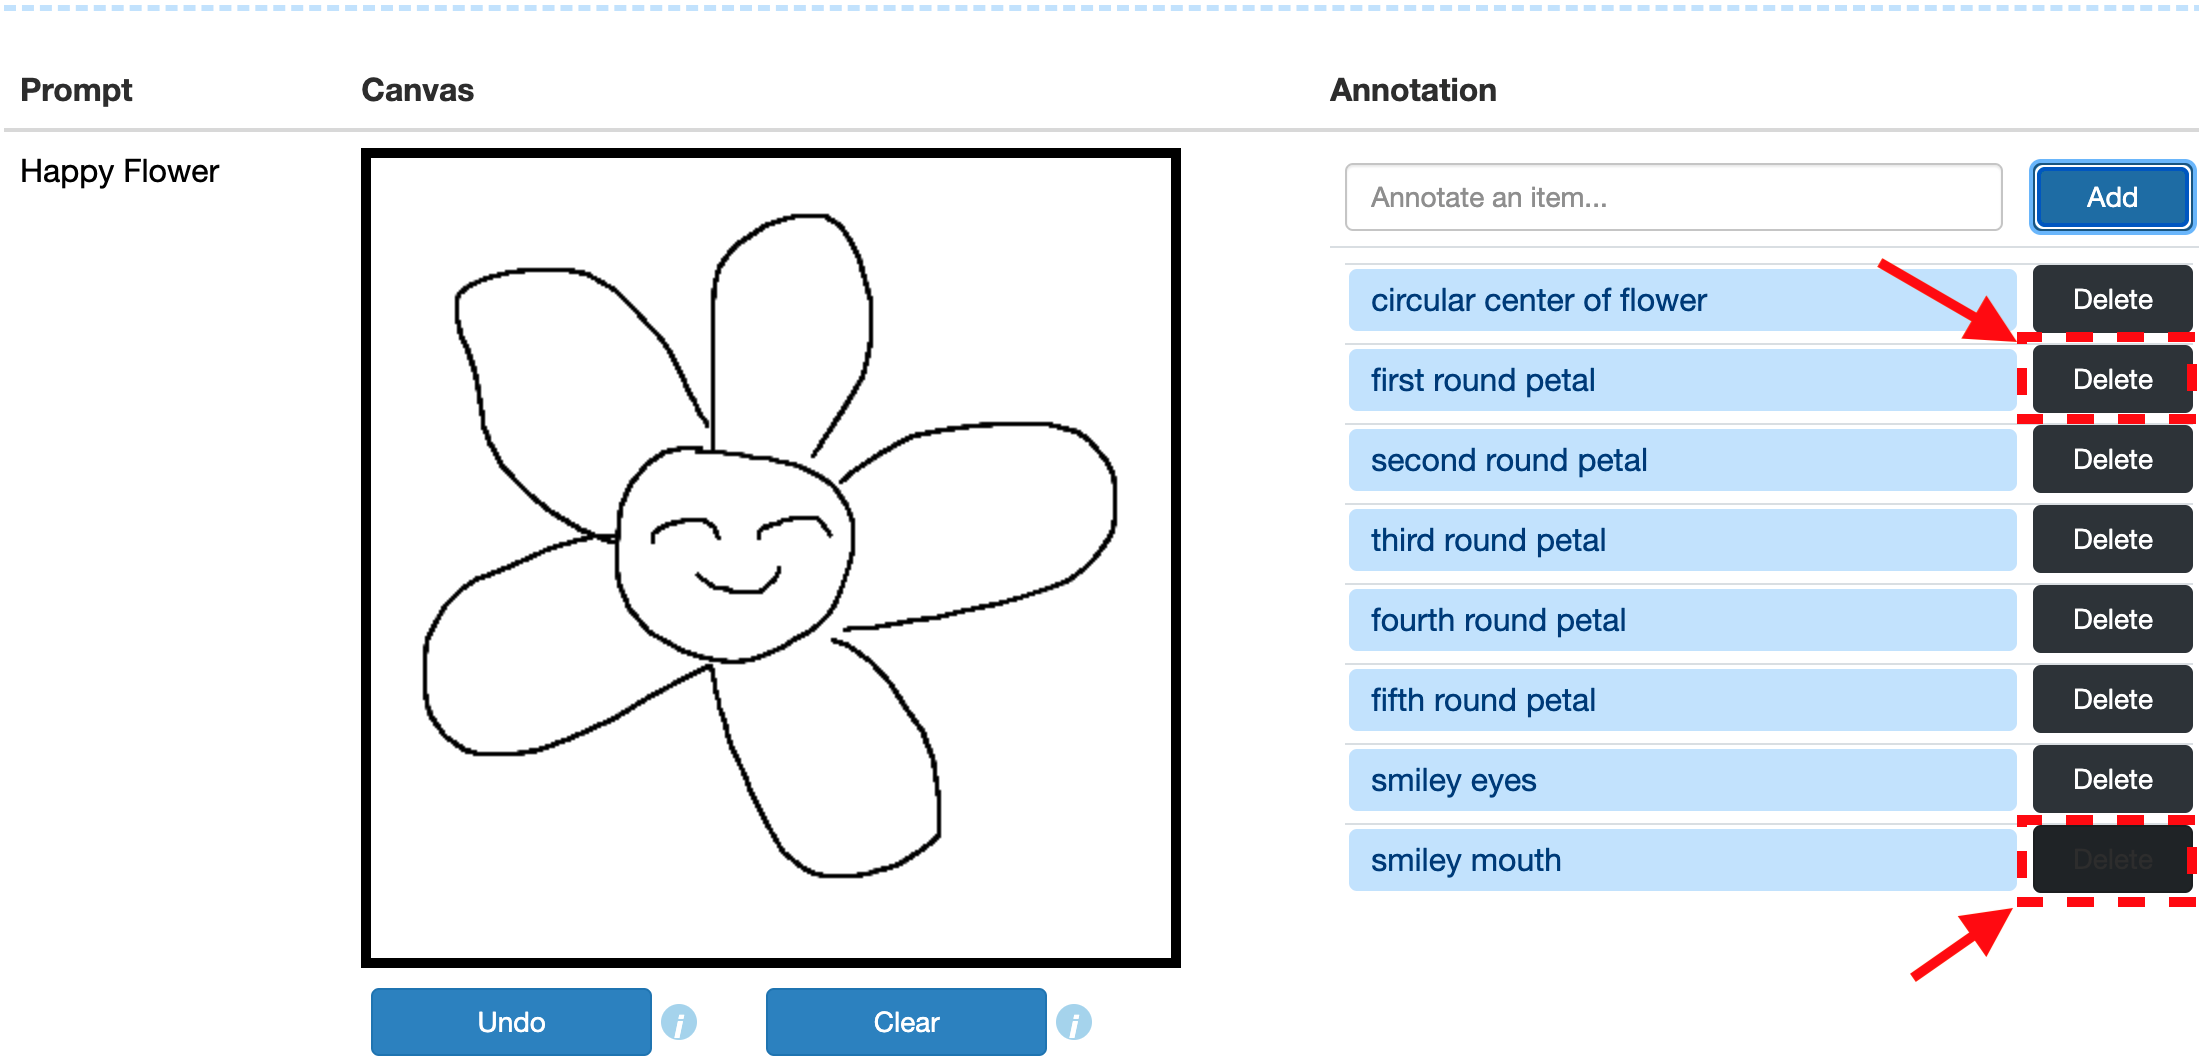
\includegraphics[width=.8\linewidth]{data_collection/v1_before_delete.png}  
\end{subfigure}
\newline
\begin{subfigure}{\textwidth}
\centering
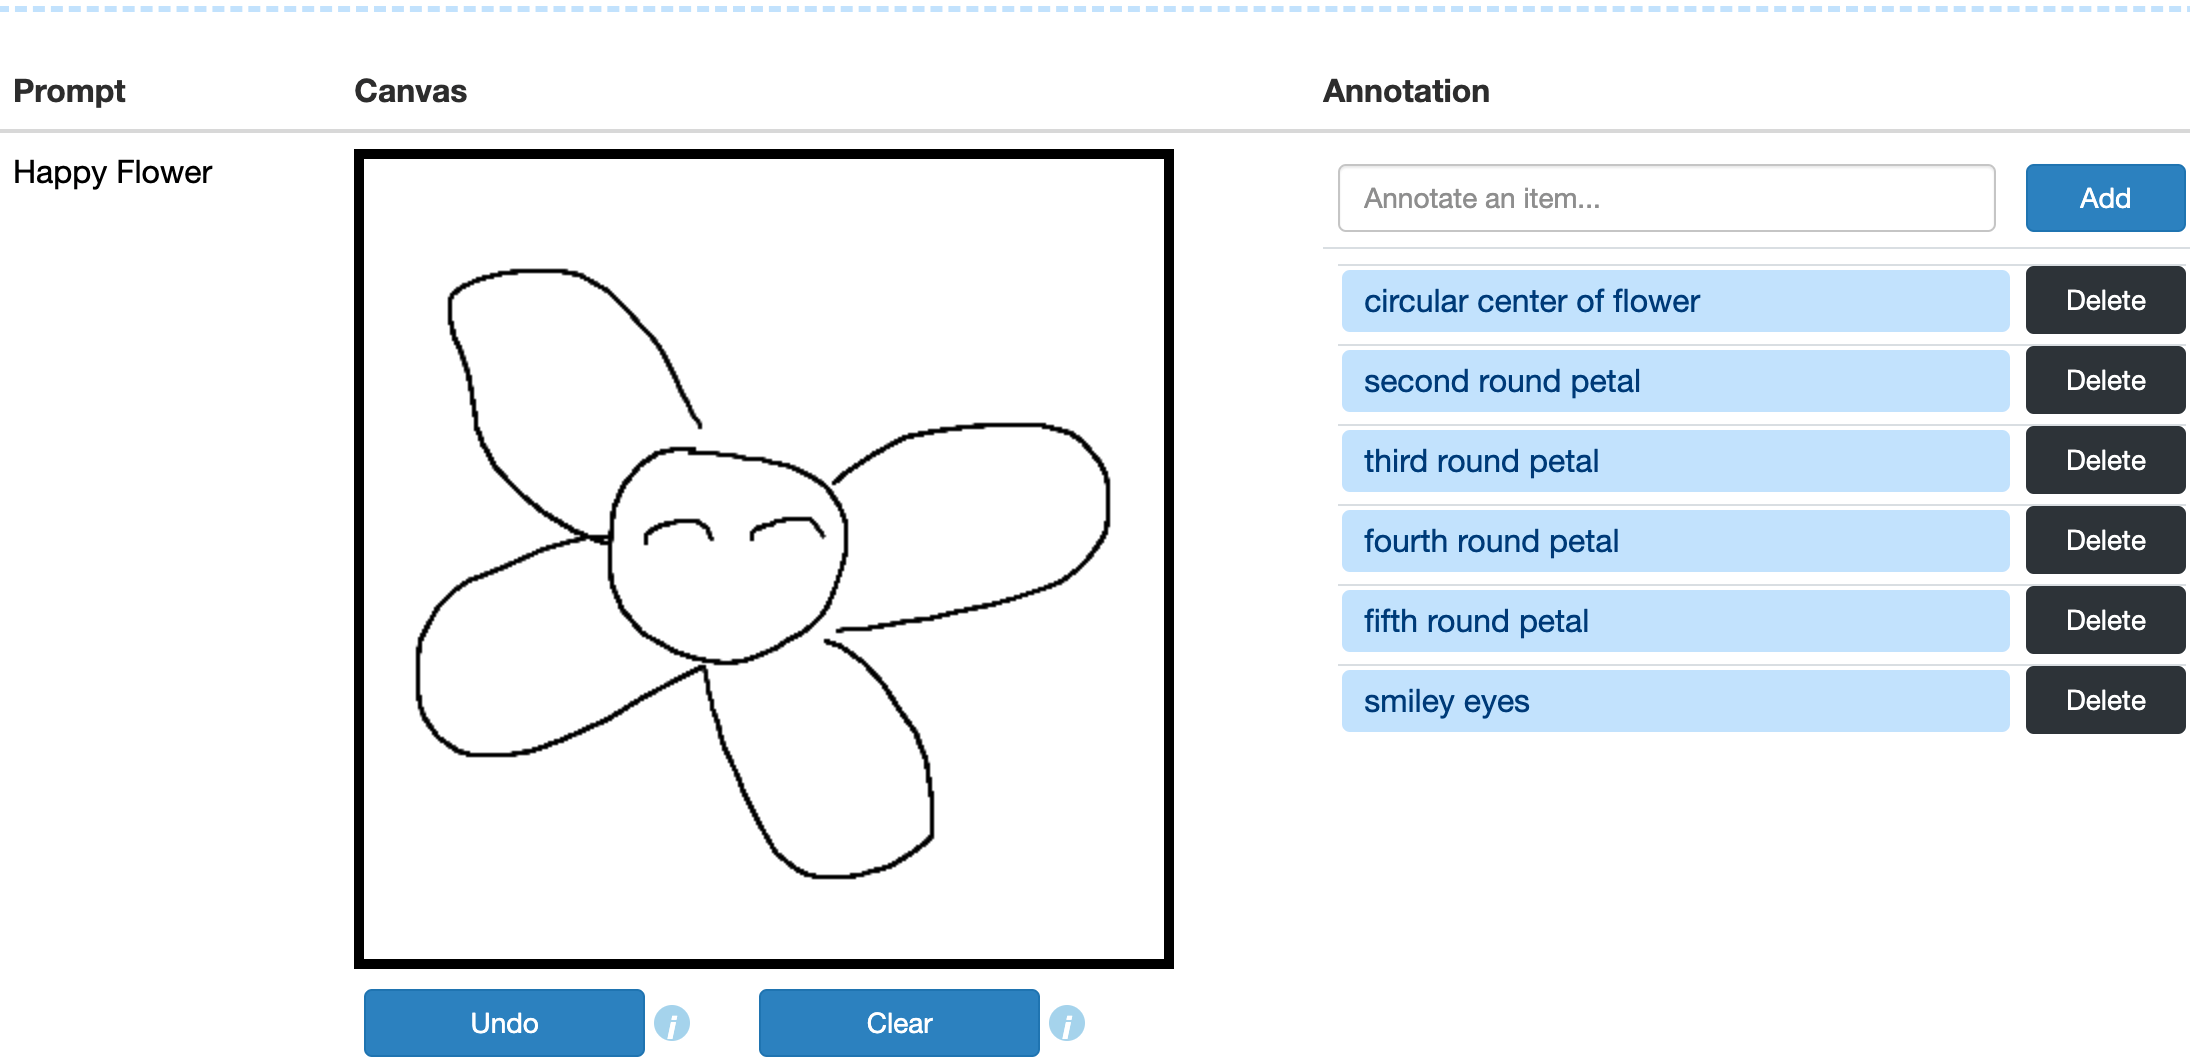
\includegraphics[width=.8\linewidth]{data_collection/v1_after_delete.png}  
\end{subfigure}
\caption{Top: the completed annotation for the prompt \textit{Happy Flower}. Red arrows and boxes point to \textit{Delete} buttons that can delete the text annotations along with their drawings. Bottom: after deleting the steps \textit{first round petal} and \textit{smiley mouth}.}
\label{v1.main_task.delete}
\end{figure*}

We illustrate a typical annotation process in Figure \ref{v1.main_task.1}. 
The annotator draws a step on the canvas, enter text description for this step in the \textit{Annotation} column, and hit \textit{Add} to display it as a new row in the annotation table. 
For the annotator's convenience, we include an \textit{Undo} button and a \textit{Clear} button for erasing strokes and clearing the entire canvas. 
If the annotator wants to remove an entire step, including the drawing and the text description, they can use the \textit{Delete} button. An example is shown in Figure \ref{v1.main_task.delete}.
Repeat the drawing-and-adding process until the drawing is done. 
This design encourages turkers to decompose their drawings into semantically meaningful parts.

We encountered some difficulties when implementing the \textit{Delete} button. At the beginning, we treated erasing strokes as drawing the same strokes but in white; however, when strokes overlap each other, overwriting with white strokes breaks other strokes into segments. Therefore, we change the drawing canvas to use layers like Photoshop, so that deleting strokes would be the same as deleting an entire layer, leaving other strokes intact.   

\subsubsection{Instruction and Requirement}

\begin{figure*}[!htb]    
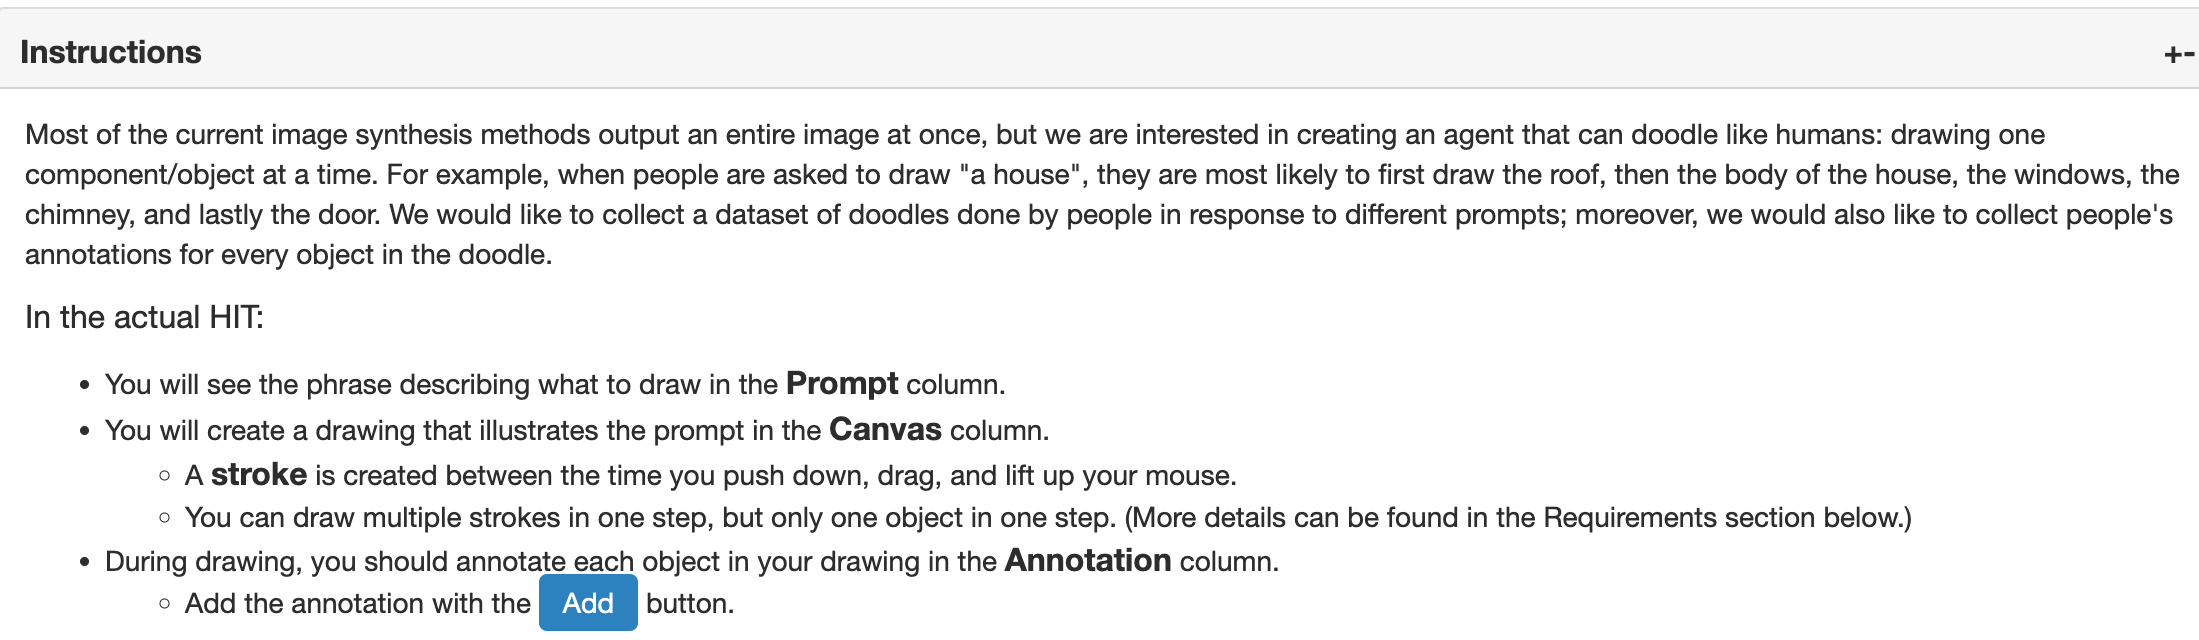
\includegraphics[width=\linewidth]{data_collection/v1_instruction.png} 
\caption{The instruction section used in the prompt-guided sketch text dataset.}
\label{v1.instruction}
\end{figure*}

To ensure that turkers understand the purpose of collecting the dataset, the instruction begins with the motivation behind this project (Figure \ref{v1.instruction}). 
What we struggled the most when drafting the requirements was deciding what a single \textit{step} in sketching was; how do we clearly explain this definition to the turkers? 
% In Version 0, we relied on common geometric shapes to decompose a drawing into a sequence of steps. 
% In Version 1, we considered asking turkers to annotate for each stroke in the drawing, but we quickly ruled out this option since it was time-consuming, and it did not align with how the instructor taught the child in the \textit{How To Draw a Cute Ice-Cream Cone} video. 
% We decided that turkers should annotate for each \textit{object} in the drawing. The ambiguity around the word \textit{object} has posed the biggest challenge in defining a clear set of requirements. 
We considered providing a list of geometric shapes, such as rectangle, triangle, circle, etc., or asking annotations for each stroke, but these options could not reflect how people naturally sketch.

There is a wide spectrum of allowed annotations depending on how people sketch. For example, when drawing for the prompt \textit{Happy Face}, one person might annotate 3 steps: \textit{large u-shaped face}, \textit{round eyes}, \textit{big smiley mouth}. But for someone who likes to draw detailed eyes, they might describe the shape of the eye contour and the length of the eyelashes. 
% So what level of specificity should be allowed?  
The great variation in personal styles makes creative sketches fascinating to study but also challenging to collect a high-quality dataset. 
% The great variation and uncertainty that comes from individuality and personal styles demonstrated through drawings would eventually drive us to not collect drawings and simply ask for text annotations for sketches found in existing datasets.  

We resorted to repeatedly testing the interface with lab mates to refine the requirements. The refinement process is explained in Appendix \ref{appendixDataV1Req}. 
The requirements deployed in the final pilot is shown in Figure \ref{v1.requirement}.
\textcolor{red}{\underline{Bad Example 2}} is shown in Figure \ref{v1.badeg} as an instance of the examples used in the final requirements. To view all the examples, refer to: \url{https://erinzhang1998.github.io/portfolio/amazon_anno}. 


\begin{figure*}[!htb]
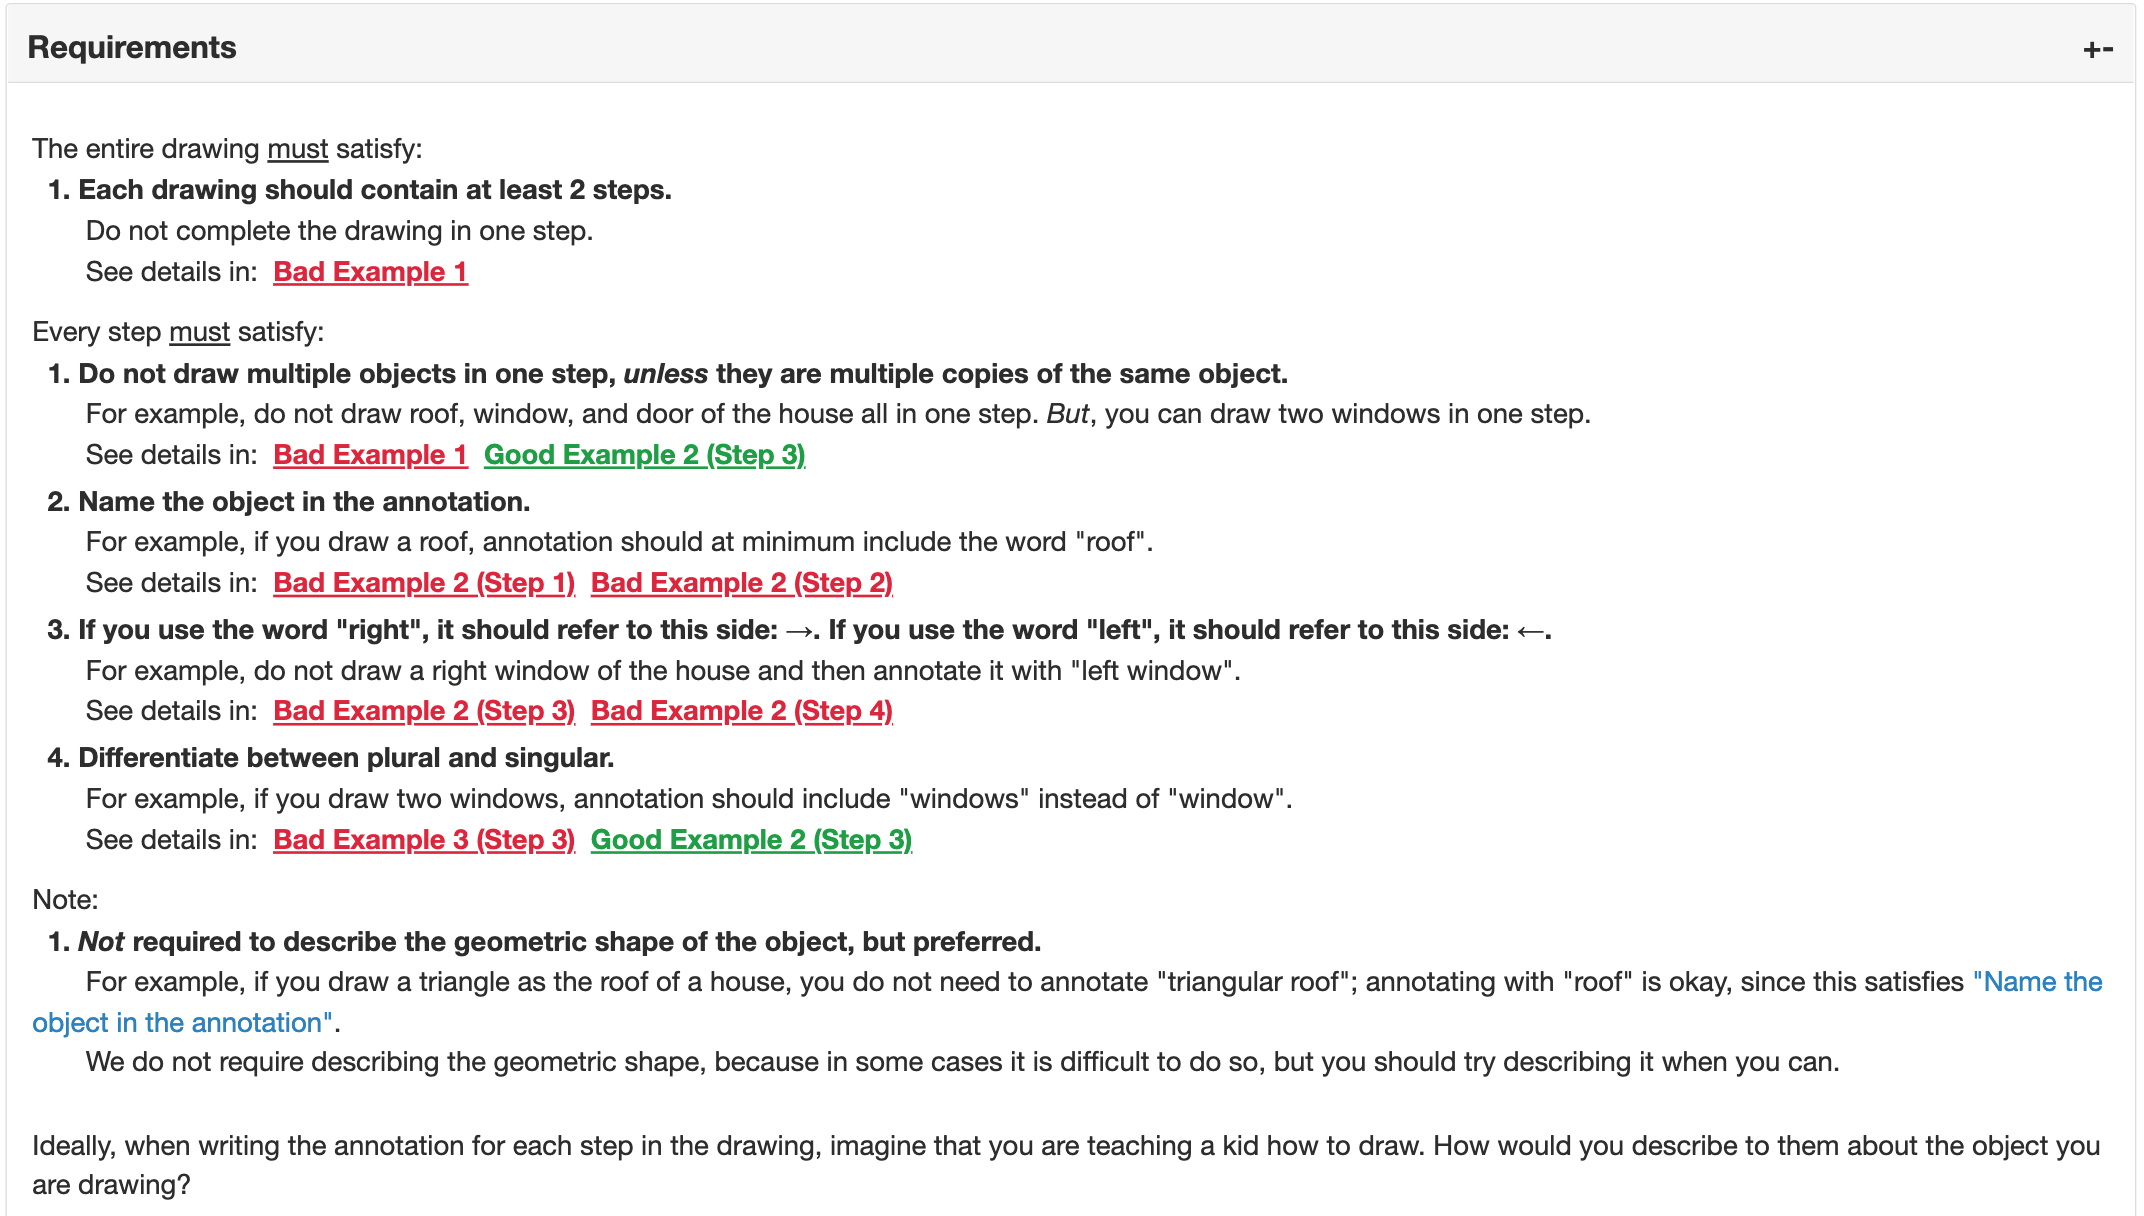
\includegraphics[width=\linewidth]{data_collection/v1_requirement.png}  
\caption{Final version of the requirements. The \textcolor{red}{\underline{Bad Example}} links to counter-examples of the requirements, and \textcolor{green}{\underline{Good Example}} links to good examples. When turkers click on the links, they are directed to the examples illustrating the corresponding requirement. This design helps them to understand the requirements better and provides high-quality annotations}
\label{v1.requirement}
\end{figure*}

\begin{figure*}[!htb]
\begin{subfigure}{\textwidth}
\centering
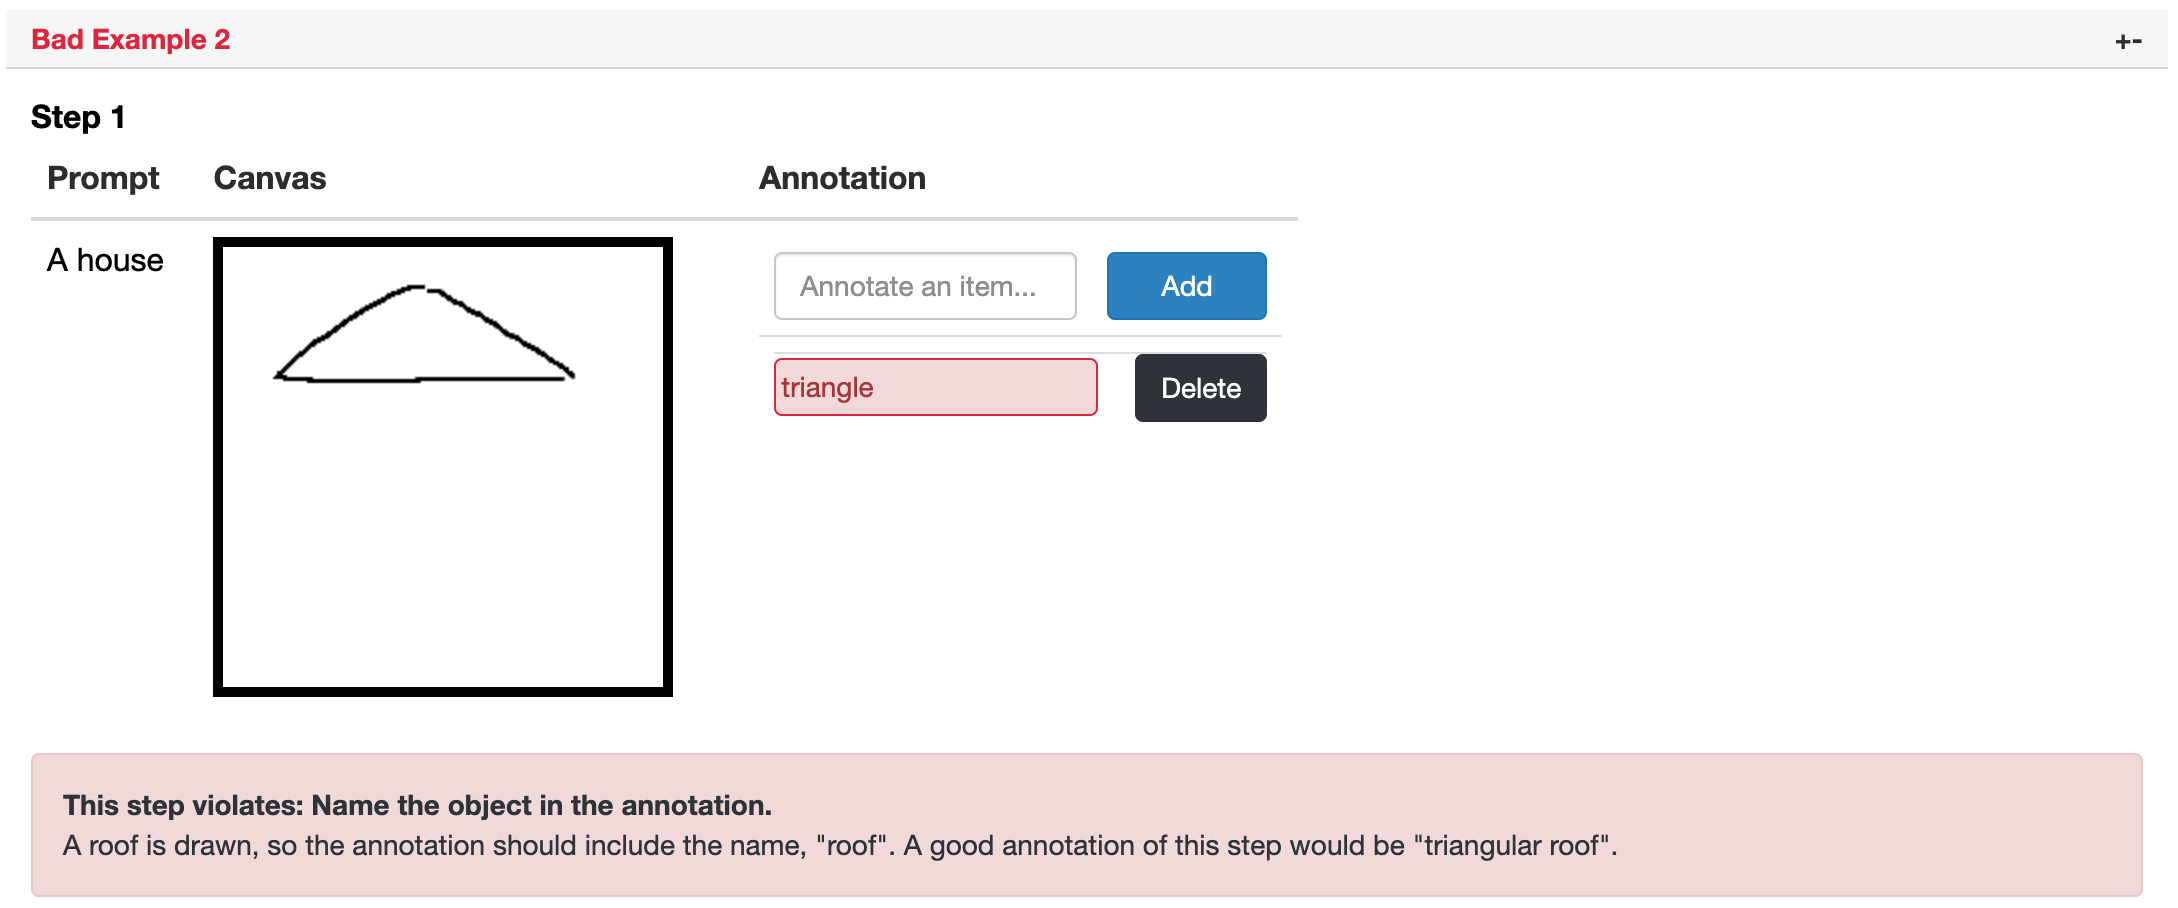
\includegraphics[width=.8\linewidth]{data_collection/v1_badeg_1.png}  
\end{subfigure}
\newline
\begin{subfigure}{\textwidth}
\centering
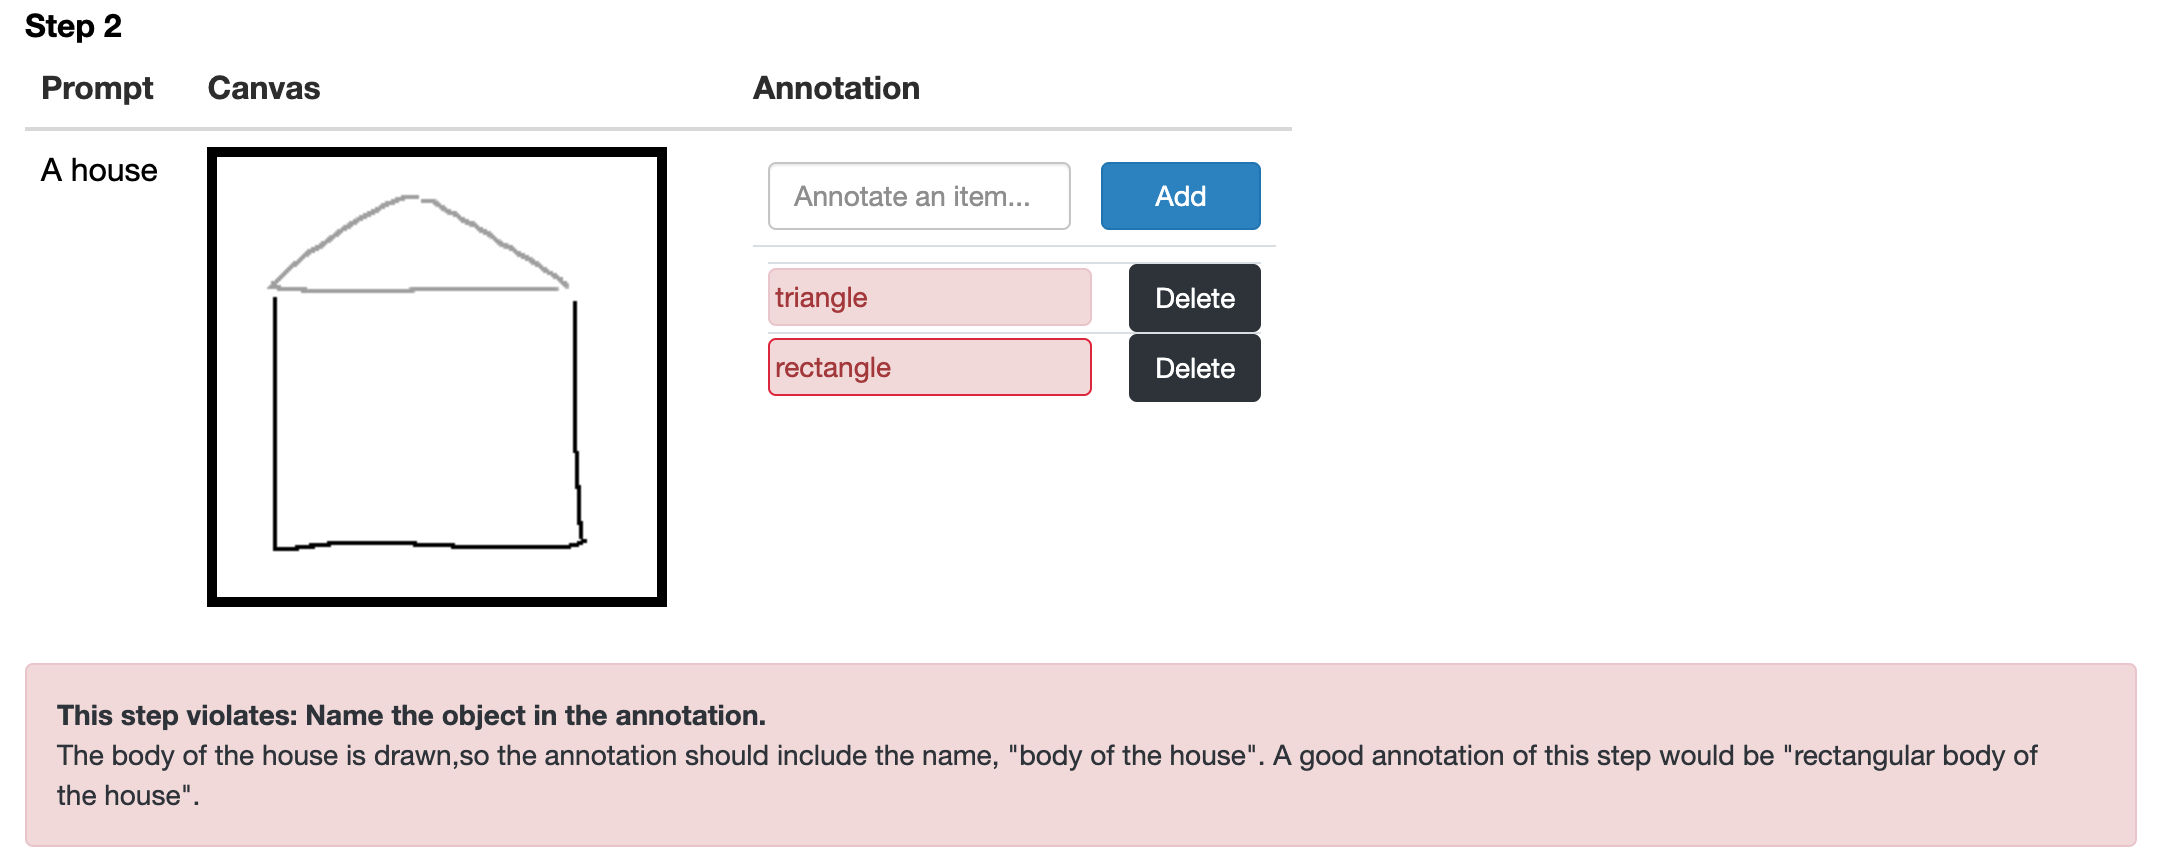
\includegraphics[width=.8\linewidth]{data_collection/v1_badeg_2.png}  
\end{subfigure}
\newline
\begin{subfigure}{\textwidth}
\centering
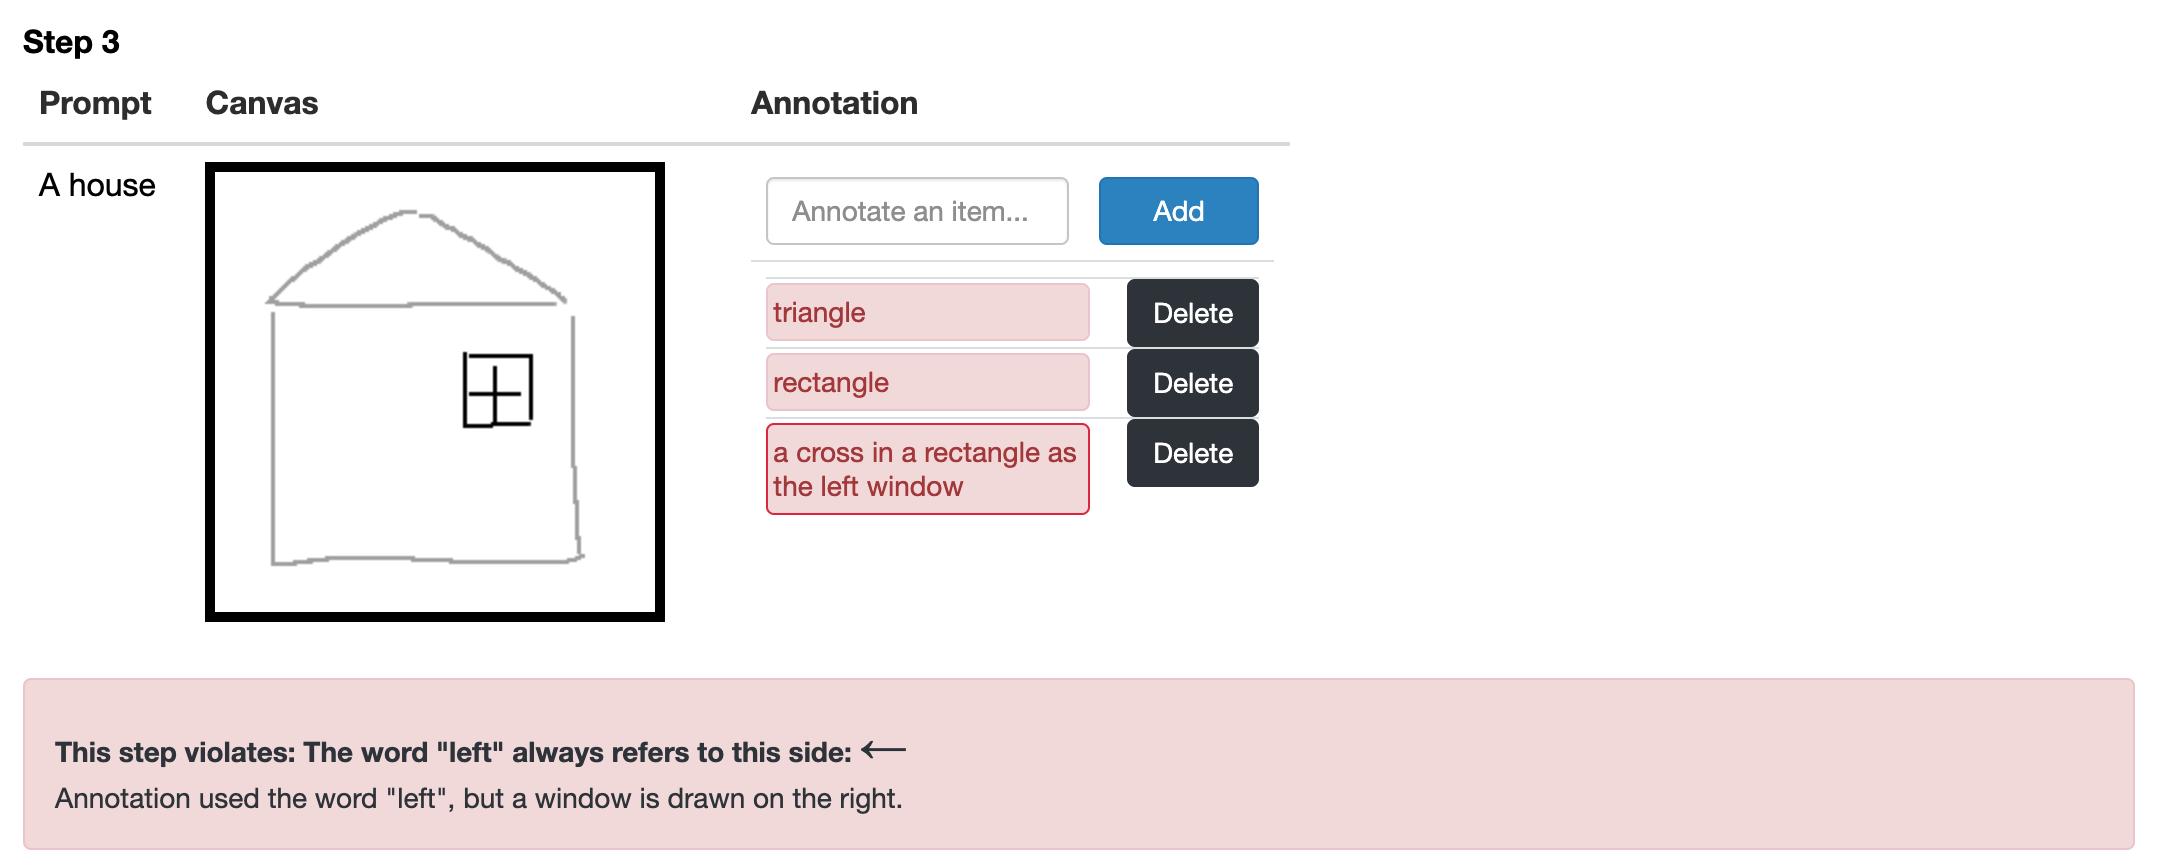
\includegraphics[width=.8\linewidth]{data_collection/v1_badeg_3.png}  
\end{subfigure}
\newline
\begin{subfigure}{\textwidth}
\centering
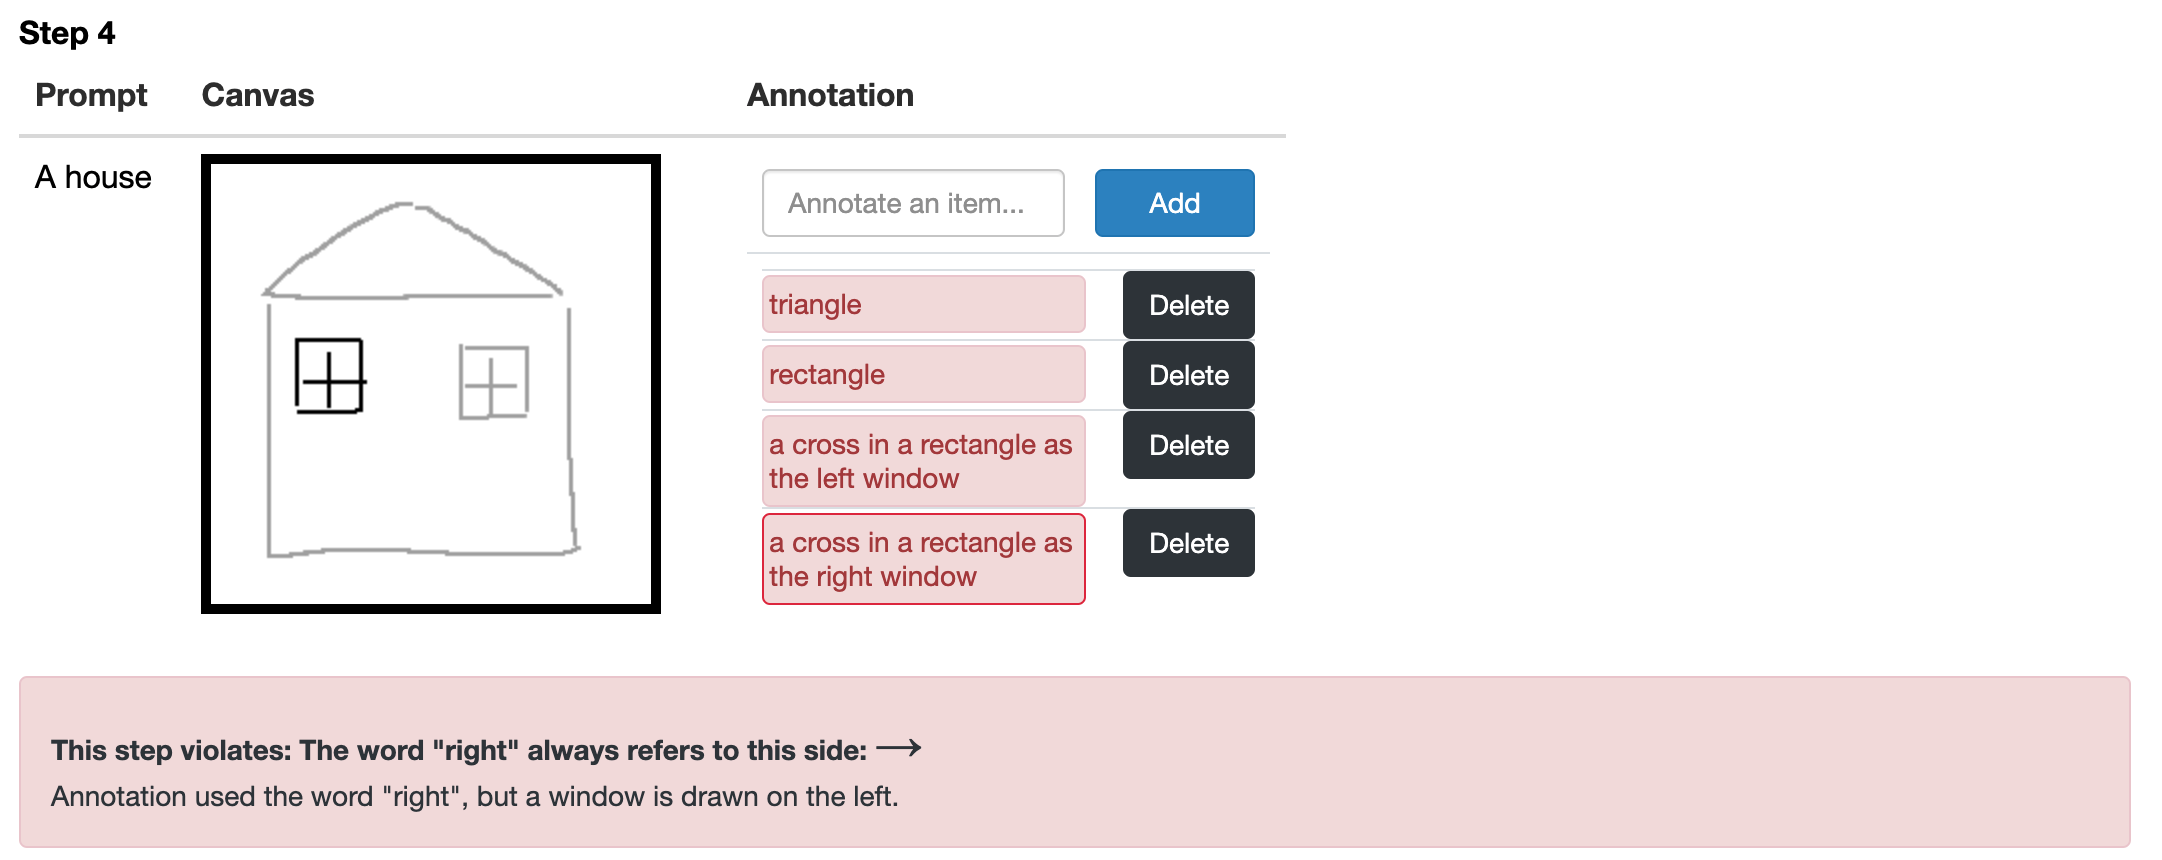
\includegraphics[width=.8\linewidth]{data_collection/v1_badeg_4.png}  
\end{subfigure}
\caption{An example used to explain the requirements to turkers.}
\label{v1.badeg}
\end{figure*}

% Most of the requirements are dedicated to ensure principle \ref{data_design_2} and \ref{data_design_3}. Requirement 1 ensures that no irrelevant sketches and trivial annotations are provided, and we resort to good faith that the annotators would provide a sketch that illustrates the given prompt. As expected, problems related to ambiguous sketches and unaligned text annotations surfaced after the deployment on AMT, eventually resulting in a complete change in format and lead to Version 2.     


\subsubsection{Qualification}



We set up a qualification test on AMT to (1) train turkers to have better understanding of the task and (2) to select turkers who can provide annotations that satisfy all the requirements. 
Similar to the process of writing the requirements, we went through several rounds of testing with students in the lab to come up with a set of questions that correspond well with the requirements. 
The qualification test starts with the same instruction and requirements in the final HIT, thus allowing turkers to familiarize themselves with the requirements and ask clarification questions before completing the actual annotation task. 
The test leads with a navigation bar (Figure \ref{v1.qualification.nav}) to make it convenient for turkers to switch between questions; originally, we displayed all questions on one page, but some found it time-consuming to scroll from the later questions back up to the instructions, so we decided to display one question at a time. 
\begin{figure*}[]
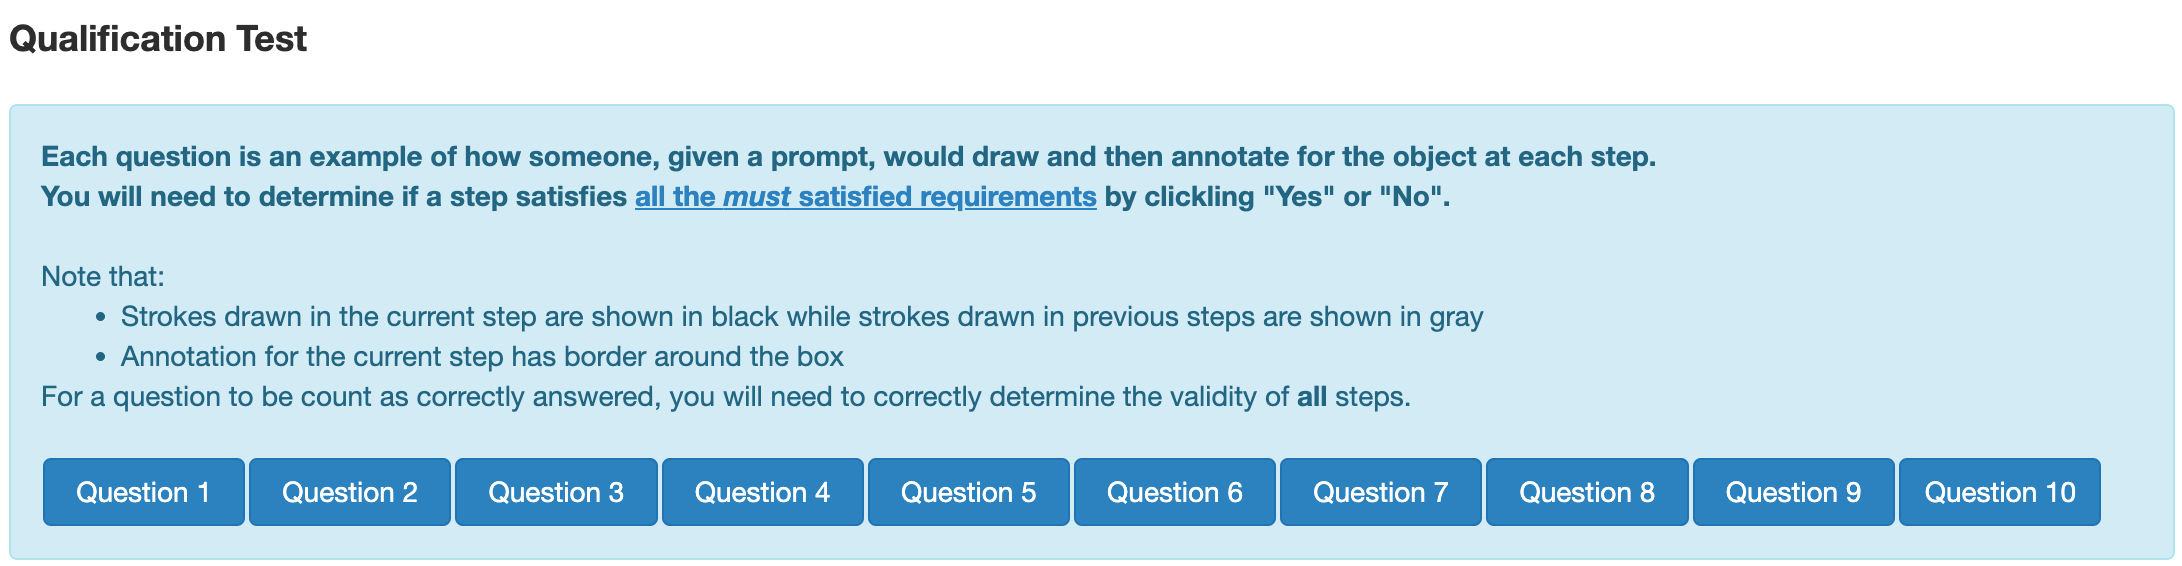
\includegraphics[width=\linewidth]{data_collection/v1_qual_header.png}  
\caption{Navigation bar in the qualification test.}
\label{v1.qualification.nav}
\end{figure*}

We show one question from the final qualification in Figure \ref{v1.qualification.q9}. 
Each question is a mock-up of the main task interface, and turkers need to determine whether every step satisfies all the requirements.
We also include hints on which requirement the question is testing to encourage turkers to revisit the requirements and form better understanding of the task.  
To see the full test, refer to: \url{https://erinzhang1998.github.io/portfolio/amazon_qual}.

\begin{figure*}[]
\begin{subfigure}{\textwidth}
\centering
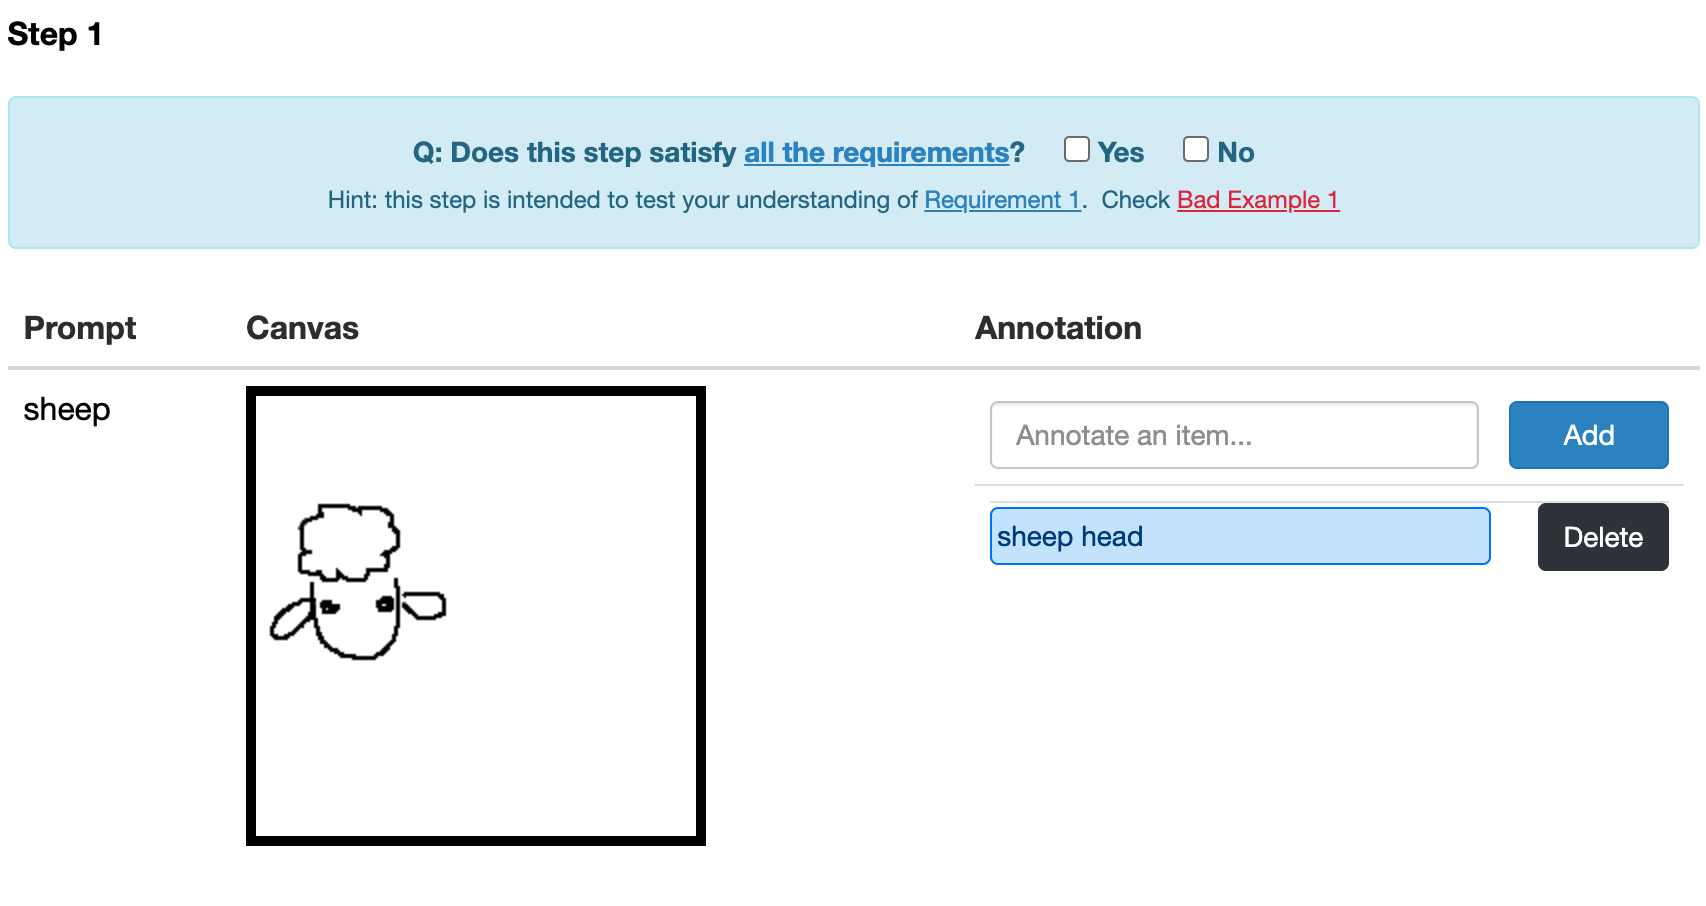
\includegraphics[width=.8\linewidth]{data_collection/v1_qual_q9_1.png}  
\end{subfigure}
\newline
\begin{subfigure}{\textwidth}
\centering
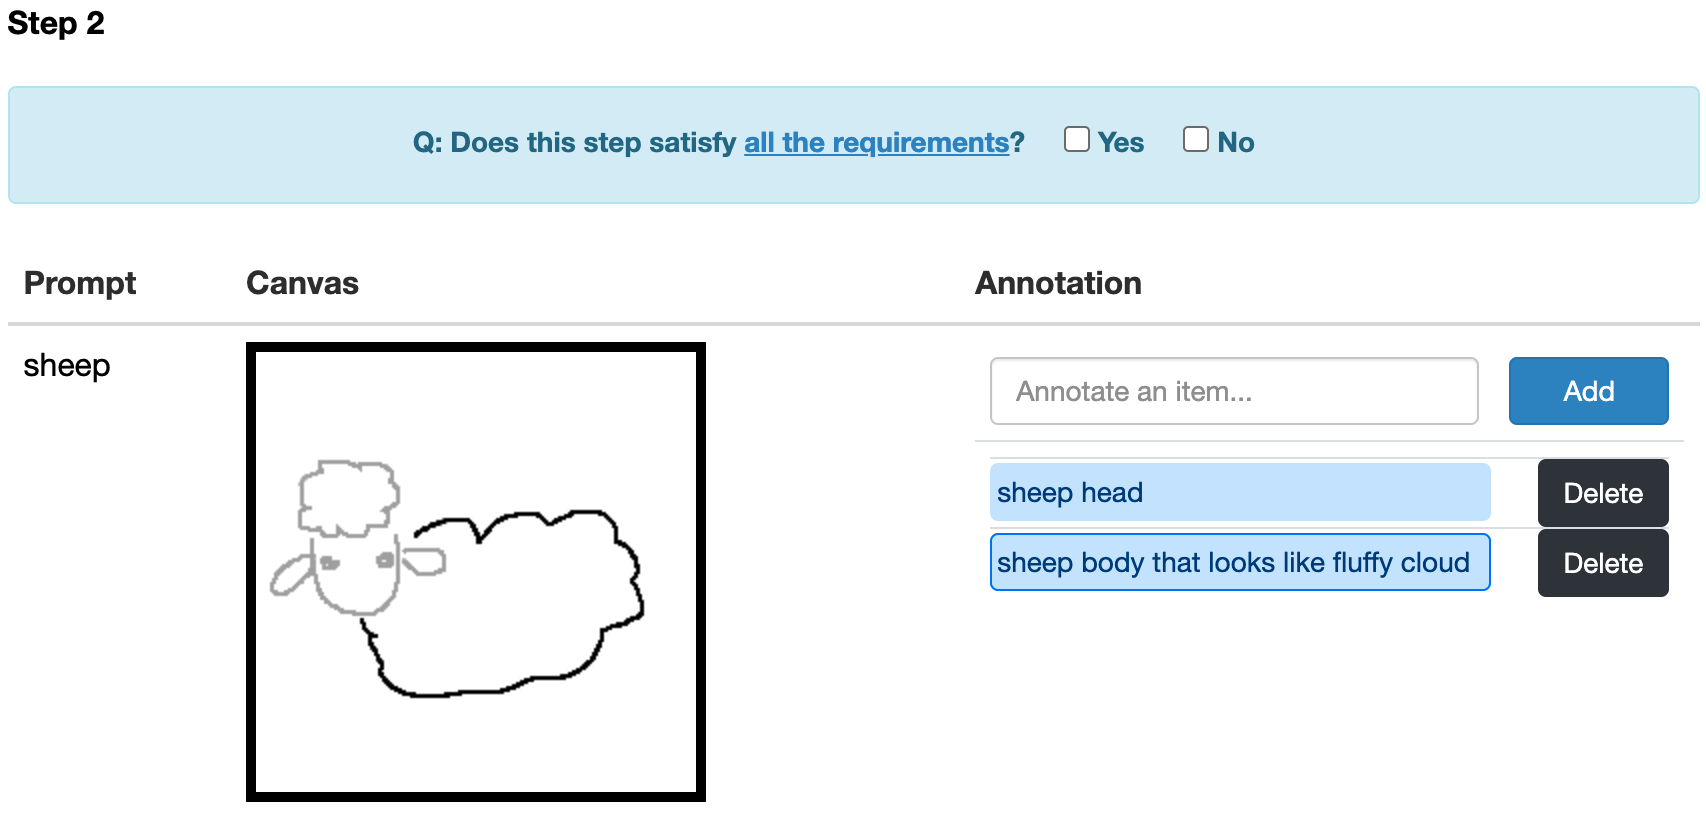
\includegraphics[width=.8\linewidth]{data_collection/v1_qual_q9_2.png}  
\end{subfigure}
\caption{An example of the questions in the qualification test.}
\label{v1.qualification.q9}
\end{figure*}

% [Figure x5: final qualification test]
%  At first, we asked the annotators to select which steps of the annotations satisfy the requirements (Figure x6.a); in order to use repetition to ensure deep understanding of the requirements, we changed to asking a yes/no question for every step, as shown in Figure x6.b.  



\subsection{Deployment Results}
% In order to determine how feasible the task is, we first deployed a version among lab members, and we obtained 55 drawings along with their annotations. All 55 drawings are shown in Figure v1.results.2. Some examples of step annotations are shown in Figure v1.results.3.  
% [Figure v1.results.2: 55 drawings from lab deployment (see jupyter notebook oct\_28\_trial\_analysis)]
% [Figure v1.results.3: 3 examples of drawings with steps?]
In our first pilot, we used prompts in the forms of \textit{adjective}$\times$\textit{noun}. 
The list of adjectives includes: \textit{happy, sad, surprised, sleepy, love-struck, evil}; the list of nouns includes: 
\textit{person, kid, cat, bear, dog, sheep, jellyfish, cup of bubble tea, apple, burger, sun, moon, star}. 
We want to see what sketches and text descriptions annotators would provide for prompts that ask for imaginative beings not in this world and include novel compositions of unrelated concepts, such as \textit{evil apple} or \textit{love-struck moon}. 
With these creative prompts, we hope to collect data that contain interesting compositions of the same geometric shapes and descriptions across different objects. 
We can then learn models that can, for example, generate circles to be different parts in different objects: eyes, moon, cherries, and angel halo. 

Since we only collected 55 sketches, we were able to manually examine every sketch, and we found many creative sketches [FIGURE]. 
However, one issue was that turkers took a long time, on average 30 minutes, to complete one sketch and provide descriptions. 

The second problem was that it was difficult to understand how some annotators interpreted the prompts through their sketches. [FIGURE]
Indeed, sketching is by its nature very subjective, a common challenge in creative AI.    

The third problem, the most concerning one, was that the part descriptions did not align well with the sketches: some annotators failed to describe every part they drew in a step, or they described parts not in the annotated step. [FIGURE]    


% [Figure v1.results.4: drawings from the amt pilot]
% [Figure v1.results.1: a: oct 28 lab deployment. b: dec 28 amt deployment]
% [Table v1.results.1: comparing the statistics of lab vs. amt deployment]
% Histograms of time each annotator spent on the task is illustrated in Figure v1.results.1. Statistics of the distributions are shown in Table v1.results.1. 
% The discrepancy might be caused by the fact that lab members with their background in computer science have implicit understandings of what kind of quality data are needed to train ML models.   